\cappar Octave es un lenguaje de programación de alto nivel. Esto
significa que es relativamente fácil hacer cosas sofisticadas con
ello.    \Octave\ es muy parecido a otro
lenguaje Matlab. Todos los comandos que utilizamos aquí de Octave
funcionan también en Matlab.
Mas informaciones sobre {\Octave} se puede encontrar en la
pagina
{\tt http://www.octave.org}.
Para la instalación del programa Octave puedes seguir las
instrucciones de la siguiente dirección
{\tt http://octave.sourceforge.net}

\begin{wrapfigure}{r}{0.6\textwidth} 
  \vspace{-20pt}
  \begin{figurebox}
    \centering
    \includegraphics[width=\textwidth]{fig1.eps}
    \caption{El gráfico de la función $f(x)=x^2$ con valores calculado
      en puntos $[-2,-1,0,1,2]$.  }
    \label{fig:1}
  \end{figurebox}
  \vspace{-120pt}
\end{wrapfigure}

\section{Octave como una calculadora avanzada}

Primeramente Octave puede ser tratada como una calculadora
avanzada. Por ejemplo, para calcular cuánto es la suma de 2 y 2. Para
esto escribimos simplemente $2+2$ y presionamos el botón {\bf Enter}.
\begin{octaveboxI}
\begin{verbatim}
 octave:1>2+2
 ans =  4
\end{verbatim}
\end{octaveboxI}
Cuando ya sabemos que 2 y 2 es 4, podemos probar algo más
complicado. Por ejemplo,
\begin{displaymath}
  \frac{(e^2-1)\cdot cos(\pi/3)}{12}  
\end{displaymath}
\begin{octaveboxI}
\begin{verbatim}
 octave:2> (e^2-1)*cos(pi/3)/12
 ans =  0.26621
\end{verbatim}
\end{octaveboxI}




\section{Gráficos 2D}

En Octave podemos asignar a una variable un valor. Por ejemplo a $x$
el valor 1204. Lo hacemos escribiendo
\begin{octavebox}
\begin{verbatim}
octave:3> x=1204
x =  1204
\end{verbatim}
\end{octavebox}


Ahora podemos calcular el cuadrado de la variable $x$ y guardarla en
otra variable $y$,
\begin{octavebox}
  \begin{verbatim}
octave:4> y=x^2
y =  1449616
\end{verbatim}
\end{octavebox}

Para dibujar el gráfico de la función $f(x)=x^2$ necesitamos calcular
los valores de la función en bastante más que un punto. Por ejemplo, en
los puntos $-2,-1,0,1,2$. Para esto definimos x como
\begin{octavebox}
\begin{verbatim}
octave:5> x=[-2 -1 0 1 2]
x =
  -2  -1   0   1   2
\end{verbatim}
\end{octavebox}

\begin{wrapfigure}{r}{0.5\textwidth} 
      \vspace{-10pt}
  \begin{figurebox}
      \centering
\includegraphics[scale=.4]{fig2.eps}
\caption{El gráfico de la función $f(x)=x^2$ con valores calculado en
  puntos $[-2, -1.9, -1.8, -1.7, -1.8, \ldots ,1.9, 2]$.  }
\label{fig:2}
\end{figurebox}
\vspace{-150pt}
\end{wrapfigure}

Ahora $x$ es un vector $[-2, -1, 0, 1, 2]$. Para calcular los valores
de la función en cada una de las coordenadas de $x$ escribimos
\begin{octaveboxI}
  \begin{verbatim}
 octave:6> y=x.^2
 y =
    4   1   0   1   4
\end{verbatim}
\end{octaveboxI}
y con esto podemos dibujar el gráfico.
\begin{octaveboxI}
  \begin{verbatim}
 octave:7> plot(x,y)
\end{verbatim}
\end{octaveboxI}


Para obtener un gráfico mejor necesitamos tener los puntos del eje $x$
mas densos. Podría ser un poco aburrido  escribir 
\begin{octaveboxI}
{\footnotesize
  \begin{verbatim}
 octave:8> x=[-2 -1.9 -1.8 -1.7 -1.8 ... 1.9 2]
\end{verbatim}}
\end{octaveboxI}
por esto, Octave tiene un comando que calcula muchos puntos de un
intervalo. Aquí queremos todos los números entre $-2$ y $2$
distanciados por $0,1$ unidades. Esto podemos obtenerlo escribiendo
simplemente
\begin{octavebox}
\begin{verbatim}
octave:9> x=-2:0.1:2;
\end{verbatim}
\end{octavebox}
Después  repetimos,
\begin{octavebox}
\begin{verbatim}
octave:10> y=x.^2; 
\end{verbatim}
\end{octavebox}
y con esto podemos dibujar un gráfico bastante mejor.
\begin{octavebox}
  \begin{verbatim}
octave:11> plot(x,y)
\end{verbatim}
\end{octavebox}

\newpage

\begin{wrapfigure}{r}{0.5\textwidth} 
      \vspace{-10pt}
  \begin{figurebox}
\centering
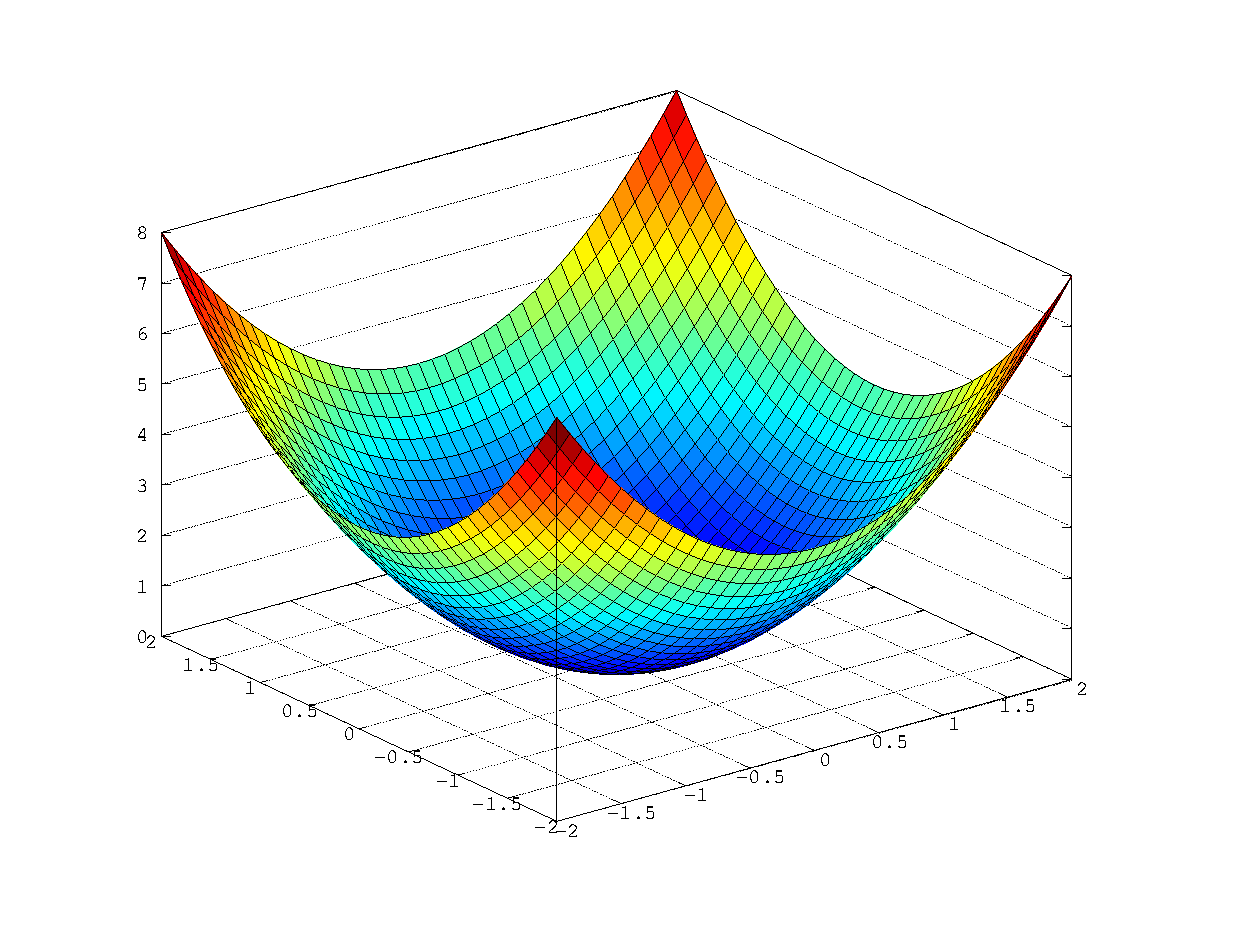
\includegraphics[scale=.4]{fig3.eps}
\caption{El gráfico de la función $f(x,y)=x^2+y^2$.}
\label{fig:3}
\end{figurebox}
\end{wrapfigure}

\section{Gráficos 3D}
Para obtener un gráfico 3D tenemos que definir una malla en el plano. Esto se realiza
\begin{octaveboxI}
{\small 
\begin{verbatim}
 octave:12> [x y]=meshgrid(-2:0.1:2,-1:0.1:1);
\end{verbatim}}
\end{octaveboxI}
Evaluamos la función en la variable z:
\begin{octaveboxI}
\begin{verbatim}
 octave:13> z=x.^2+y.^2;
\end{verbatim}
\end{octaveboxI}
y dibujamos
\begin{octaveboxI}
\begin{verbatim}
 octave:14> surf(x,y,z);
\end{verbatim}
\end{octaveboxI}
Para grabar el gráfico en el formato eps
\begin{octaveboxI}
\begin{verbatim}
 octave:13> print fig.eps
\end{verbatim}
\end{octaveboxI}

\vspace{3cm}
\noindent
\includegraphics[width=\textwidth]{pubmm2.png}

\newpage
%%% Local Variables: 
%%% mode: latex
%%% TeX-master: "informaticaeningenieria"
%%% End: 



